% SEE: https://solid.iis.fraunhofer.de/SCS-DS-IoT/public/2024/solid%20symposium/index.html
% 4 pages + reference
% AFTER review 2 extra pages allowed
% Deadline 29/03

\documentclass[
% twocolumn,
% hf,
]{ceurart}

%%
%% One can fix some overfulls
\sloppy

%%
%% Minted listings support 
%% Need pygment <http://pygments.org/> <http://pypi.python.org/pypi/Pygments>
\usepackage{minted}
%% auto break lines
\setminted{breaklines=true}
\usepackage[labelfont=bf,format=plain, 
justification=raggedright,singlelinecheck=false]{caption}
\usepackage[hidelinks]{hyperref}

\newcommand{\dquote}[1]{``#1''}
\newcommand{\squote}[1]{`#1'}
\newcommand{\code}[1]{\texttt{#1}}

%%
%% end of the preamble, start of the body of the document source.
\begin{document}

\copyrightyear{2024}
\copyrightclause{Copyright for this paper by its authors. Use permitted under Creative Commons License Attribution 4.0 International (CC BY 4.0).}
\conference{The 1st Solid Symposium Poster Session, co-located with the 2nd Solid Symposium, May 02 -- 03, 2024, Leuven, Belgium} % I know there is an overfull, but this is the latex that they provide

\title{Discoverable and Interoperable Augmented Reality Environments Through Solid Pods}


\author{Maxim {Van de Wynckel}}[%
orcid=0000-0003-0314-7107,
email=mvdewync@vub.be,
url=https://maximvdw.be/profile/card,
]
\cormark[1]
\address{Web \& Information Systems Engineering Lab, Vrije Universiteit Brussel, 1050 Brussels, Belgium}

\author{Beat Signer}[%
orcid=0000-0001-9916-0837,
email=bsigner@vub.be,
url=https://beatsigner.com,
]


\begin{abstract}
    Augmented Reality~(AR) environments are physical environments with virtual objects superimposed through AR-enabled devices. These virtual objects can range from simple aesthetic objects such as pictures to superimposed contextual information about physical items. In most modern AR~applications, these augmented spaces exist only for the user who created the environment or for proprietary applications that enable multi-user collaboration in the same environment. However, there is a lack of solutions that enable interoperable collaboration in these personal AR~spaces, allowing users to share and contribute to an AR~space. We propose a solution that enables users to create their personal AR~space that can then be discovered by other users who are in physical proximity to this space, enabling them to view or contribute to the augmented space. In addition, we discuss a solution that utilises the same technique to create AR~spaces that are bound to a specific room and can be discovered by users who are in close vicinity to these rooms.
\end{abstract}
\begin{keywords}
  Solid \sep
  Augmented Reality \sep
  Physical Pod Discovery \sep
  AR Collaboration
\end{keywords}

\maketitle
\section{Introduction and Related Work}
In Augmented reality~(AR), virtual objects are superimposed onto the physical world. Since its early days, AR has significantly advanced to portable devices such as smartphones and head-mounted displays~\cite{10.5555/2427126}, enabling its use in regular environments such as office buildings to superimpose virtual information to the physical world.

Superimposed virtual objects or information can be anchored to physical objects and walls within these physical environments~\cite{10.1145/3301275.3302278,kalaitzakis2021fiducial}. These virtual objects can range from textual information such as timers or instructions to images, videos or interactive elements~\cite{6948506}. However, there is a lack of AR solutions that enable collaboration on the creation of these AR environments without the need for proprietary applications.

A conceptual content sharing solution for AR, offering a peer-to-peer and client-server collaboration solution using events that indicate changes to the virtual objects, was proposed in~\cite{236306}. While this solution supports collaboration in AR, it still requires a complex communication framework and does not tackle the problem of different devices using a different frame of reference~\cite{mou2004frames}.

We propose an interoperable solution that enables users to create their personal AR environments that can be discovered in the physical world by other users using AR-enabled devices. Unlike existing work~\cite{10.1145/3567721}, we aim for an interoperable solution that decentralises the collaborative aspect of AR environments, while also enabling the sharing of crucial environmental information such as common reference spaces.
\section{Solution}
The goal of our proposed solution is to allow multiple AR devices to contribute to a single shared AR environment or virtual space belonging to a user. We assume that the AR device used to contribute to augmented environments is a smart device that has access to the Web and can broadcast an RF signal. In the general architecture of our proposed solution, we let AR devices broadcast a semantic Bluetooth Low Energy~(BLE) beacon advertisement containing the URI of a specific resource. We utilise the advertising protocol of SemBeacon~\cite{10.1145/3627050.3627060} that advertises an AltBeacon advertisement and Eddystone-URL compatible scan response to broadcast semantic data URIs. In addition, SemBeacon has a BLE~v5.0 advertisement that prevents the need to shorten the URI to fit within the PDU. The use of SemBeacon to advertise the environment URI is illustrated in \figurename~\ref{fig:architecture}. This environment resource contains information about the personal environment(s) owned by the user. Other devices can receive these advertisements when in proximity to the AR device and then access the URI to retrieve more information. For each environment, we have a link to a public inbox that can be used by other users to link their own modifications to the environment. Any modifications made to the superimposed space are stored in a Solid Pod owned by the user who made the modifications, which enables users to both contribute to the same environment as well as control the access rights of modifications made to these environments.

\begin{figure}[h]
    \centering
    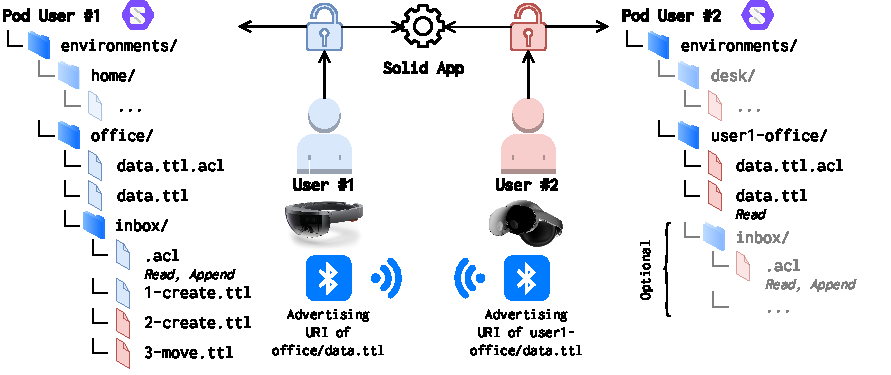
\includegraphics[scale=0.90]{images/sosy_architecture.pdf}
    \caption{A user's discoverable AR environments with two example users (\#1 and \#2) having a Solid Pod}
    \label{fig:architecture}
\end{figure}

On the left-hand side of the architecture shown in \figurename~\ref{fig:architecture}, we have a Solid Pod for user~1. The Pod contains all environments owned or modified by the user. An AR device connects to the user's Solid Pod through a Solid application that authenticates the user, allowing it to modify the resources when editing a virtual environment. In order to enable the discovery of these virtual spaces, the AR device broadcasts the \texttt{*.ttl} file of the environment it is currently in via BLE advertisements. This resource contains all the information about the environment, such as its location, any identifiable features and all virtual objects placed relative within this environment. While the URI that is broadcasted is public, the access to read this URI is controllable through access control lists implemented in Solid. SemBeacon offers a broadcasted flag to indicate if a URI is publicly accessible to prevent applications that do not have access to the resource from attempting to access it.

When another user (e.g.~user~2) wants to modify the environment of user~1, they create a new resource including the modifications and additions to virtual objects or detectable features (e.g.~markers). The application will then notify user~1 about these changes by referencing the \texttt{user1-office/data.ttl} file in the \emph{inbox}~\cite{10.1007/978-3-319-58068-5_33} container of the environment that is being modified. Solid also enables the access rights of these modifications, more information about access control for environments and modifications is provided in Section~\ref{subsec:access}.

\begin{figure}[htb]
\begin{minipage}{1\columnwidth}
\begin{minipage}{.44\columnwidth}
\centering
    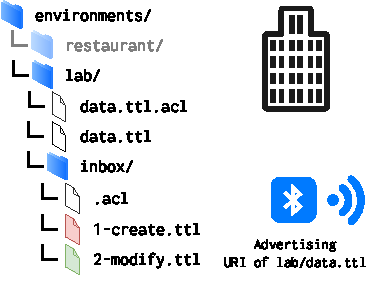
\includegraphics[scale=0.90]{images/sosy_architecture_2.pdf}
\end{minipage}
\begin{minipage}{.55\columnwidth}
\begin{minted}[xleftmargin=5pt,fontsize=\small]{turtle}
<> a seas:Room ; rdfs:label "Our Lab"@en ;
  ldp:inbox <./inbox/> ;
  vcard:address [ ... ] .
:printer_marker a fidmark:AruCo ;
  fidmark:markerIdentifier 12 .
:printer_info a sosa:FeatureOfInterest ;
  poso:hasPosition [ 
    poso:isRelativeTo :printer_marker ;
    ... ] ;
  omg:hasGeometry [ ... ] .
\end{minted}
\end{minipage}
\caption[Single discoverable AR environment]{Single discoverable AR environment using the 
\code{seas}\footnote{Smart Energy Aware Systems Ontology: \url{https://w3id.org/seas/}}, \code{fidmark}\footnote{Fiducial Marker Ontology: \url{http://purl.org/fidmark/}}, \code{poso}\footnote{Positioning System Ontology: \url{http://purl.org/poso/}} and \code{omg}\footnote{Ontology for Managing Geometry: \url{https://w3id.org/omg\#}} vocabularies}
\label{fig:architecture_2}
\end{minipage}
\vspace{-0.1cm}
\end{figure}

An alternative architecture is illustrated in \figurename~\ref{fig:architecture_2}. In this scenario, a fixed Bluetooth beacon is placed in a room, broadcasting the URI of a single environment. This scenario can be used for public physical environments, such as a meeting room or laboratory, enabling collaboration in AR. Similar to personal environments shown in \figurename~\ref{fig:architecture}, users store their changes to an environment in their Solid Pod and reference these changes in the inbox of the environment.

\subsection{Usage} \label{subsec:usage}
Our solution is depicted in \figurename~\ref{fig:flow} where we showcase the flow of our architecture previously illustrated in \figurename~\ref{fig:architecture}. Two users with AR devices have their own Solid Pod. User~1 will create an environment ($A$) on their Pod and subscribe to the inbox container of this environment. Once the environment is ready, the AR device will use the SemBeacon specification to advertise the URI of the environment to enable its discovery.

\begin{figure}[htb]
\centering
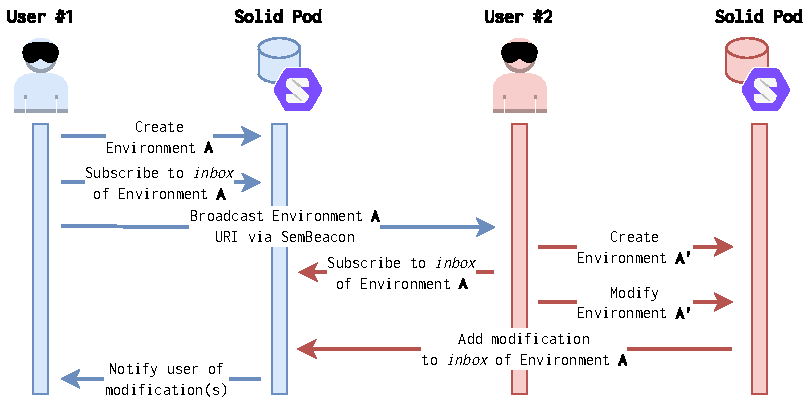
\includegraphics[scale=0.90]{images/flow.pdf}
\caption{Interaction flow of two users contributing to the same augmented reality environment} \label{fig:flow}
\end{figure}

When another user, such as user~2 discovers the resource URI the AR application will access the environment to visualise the augmented objects. If user~2 makes a modification such as adding virtual objects, these modifications are stored in the Pod of user~2 as environment $A'$, ensuring ownership of this contribution and enabling user~2 to choose the access rights to this modification. To keep up-to-date with changes in the original environment, the application will listen for changes in the inbox of environment $A$. All users who are subscribed to this inbox will receive notifications whenever a new modification is added.

An inbox uses the LDP\footnote{\url{https://www.w3.org/ns/ldp\#}} vocabulary to index all resources within this container. A user who wishes to accept contributors for their environment should configure this inbox container with public \textit{append} access rights, giving other users the opportunity to append a new resource to the container. Each inbox item represents an action using the \mbox{schema.org} vocabulary~\cite{10.1002/asi.24744}.

\begin{listing}[htb]
\begin{minted}[xleftmargin=5pt,fontsize=\small]{turtle}
@prefix card: <https://user2.solidweb.org/profile/card#> .
@prefix office: <https://user2.solidweb.org/environments/user1-office/data.ttl#> .

<> a schema:CreateAction ;
  schema:description "Created a new object 'painting' with label 'User 2'"@en ;
  schema:agent <https://ar-app.com/id> ;  # AR application that created the action
  schema:creator card:me ;                # Owner of the modification
  schema:object office:painting ; schema:result office:painting .
\end{minted}
\caption{Inbox item to identify the creation of a virtual object} \label{lst:inbox-example}
\end{listing}

Listing~\ref{lst:inbox-example} demonstrates an individual appended inbox item to the Solid Pod of user~1. In the example we see a \code{schema:CreateAction} indicating that user~2 created a new \textit{painting} object. Users can listen for notifications in the inbox to automatically apply changes to virtual objects in the shared AR environment as they are made~\cite{10.1007/978-3-319-58068-5_33}.

Positioning virtual objects is done using the POSO ontology~\cite{10.1007/978-3-031-19433-7_14}, which allows the description of (virtual) objects to be placed relative to other objects using the \code{poso:isRelativeTo} predicate. When a user wants to place an object in an environment using an absolute position that is not relative to a marker or detectable feature, the same predicate can be used to indicate that the absolute position is relative to the environment.

The final AR environment combining all modifications made by other users is created by the AR application that has access to the Solid Pod. Our architecture allows users to easily ignore all contributions of another user or agent. Individual modifications or contributions can be rejected by ignoring the individual inbox items where these changes are referenced. Future work might address the moderation of individual contributions by applying quality assessment crowdsourcing techniques~\cite{10.1007/978-3-642-41338-4_17}.

\subsection{Reference Frame}
AR uses one or more reference frames~\cite{mou2004frames} to anchor virtual objects in the physical environment and to determine an absolute or relative position. This can be done through feature detection~\cite{10.1145/3301275.3302278} that creates anchors based on visual patterns or artificial features such as fiducial markers~\cite{kalaitzakis2021fiducial}.

In order to enable interoperable applications to contribute to the same environment, all applications need to operate within the same reference frame. Our solution assumes that contributions to an environment not only include virtual objects, but also additional anchor points such as markers and detectable features that are contributed by multiple users~\cite{fidmark}. By semantically describing these reference frames as objects on itself, the POSO ontology can be used to position virtual objects relative to these anchors.

\subsection{Access Control} \label{subsec:access}
Solid enables users to have control over the access rights of their data and resources. In the scope of our solution, this entails the data that is shared in the AR environment (i.e.~virtual objects and anchors) by both the user who owns the environment and other users who make that own modifications to the environment.

Each modification to an environment is made in the Solid Pod of the user who made the modification, giving them full control on the access rights to these modifications -- as well as control on the actions which are normally created in the original environment to notify the original owner of the environment (see Section~\ref{subsec:usage}).
\section{Conclusion and Future Work}
We presented a solution enabling the collaboration and sharing of personal augmented reality~(AR) environments by using Solid Pods. Our solution allows these personal AR spaces to be discoverable within the physical space that these environments are augmenting by means of semantic beacons that advertise a URI~\cite{10.1145/3627050.3627060}. While our proposed solution allows users to choose which collaborators to accept for the environment through the inbox system, it is currently impossible to accept individual contributions from a single collaborator. Future work might address this issue by applying crowdsourcing techniques~\cite{10.1007/978-3-642-41338-4_17} to the data that is produced by other users.

While we focused on the passive discovery using BLE advertisements to enable seamless discovery of the linked data, similar architectures can be designed using other discovery methods such as a QR-code on the door of the environment. 

In the future, we might evaluate the performance differences between keeping multiple \textit{versions} of a virtual environment in different Pods (as proposed in our solution) versus using a stream of events that indicate changes to the environment, similar to the proposed work in~\cite{01H1940MY7FSFV0W0J44E3CCX7}.

\bibliography{main}

\end{document}
